\documentclass[border=20pt]{standalone}
\usepackage[american]{circuitikz}
\usepackage{amsmath}%To allow \cfrac macro
\usepackage{bm}%Bold math
\usetikzlibrary{arrows.meta,decorations.markings}

\begin{document}
    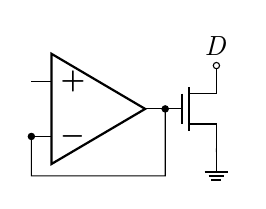
\begin{tikzpicture}
\ctikzset{bipoles/length=1cm}
\draw
(0, 0) node[op amp,yscale=-1] (opamp) {}
(opamp.-) to[short,*-] ++(0,-0.5) coordinate (leftC)
to[short,-] (leftC -| opamp.out)
to[short,-*] (opamp.out)
(1.5,0) node[nmos](mos){}
(opamp.out)to (mos.base) 
(mos.source)to (1.5,-0.5) node[ground]{}
(mos.drain) node[anchor=south] {\textit{D}} to [short,-o](1.5,0.55) ;
    \end{tikzpicture}
\end{document}